\section{Типы компиляции}
\label{sec:compilation}

Дистрибутив языка зависит от типа процессора и операционной системы. В
дистрибутив Objective CAML для каждой архитектуры (пара: процессор, операционная
система) входит интерактивная среда интерпретатора, байт--код компилятор, и, в
большинстве случаев, компилятор машинного кода для данной архитектуры.

\subsection{Названия команд}
\label{subsec:command_names}

В таблице \ref{tbl:commands_for_compiling} приводятся названия различных
компиляторов, входящих в дистрибутив Objective CAML. Первые четыре из них
являются частью каждого дистрибутива.

\begin{table}
	\begin{tabular}{|l|l|}
	\hline
	\texttt{ocaml} & интерактивная среда интерпретатора \\
	\hline
	\texttt{ocamlrun} & интерпретатор байт--кода \\
	\hline
	\texttt{ocamlc} & компилятор в байт--кода \\
	\hline
	\texttt{ocamlopt} & компилятор машинного кода \\
	\hline
	\texttt{ocamlc.opt} & оптимизированный компилятор байт--кода \\
	\hline
	\texttt{ocamlopt.opt} & оптимизированный компилятор машинного кода \\
	\hline
	\texttt{ocamlmktop} & конструктор новых сред интерпретатора \\
	\hline
	\end{tabular}
	\caption{\label{tbl:commands_for_compiling}Команды
компиляции}
\end{table}

Оптимизированные компиляторы были сами скомпилированы компилятором машинного
кода, при этом получается более быстрый исполняемый файл.

\subsection{Элементы компиляции}

Элемент компиляции соответствует наименьшей части программы на Objective CAML,
которая может быть скомпилирована. Для интерактивного интерпретатора таким
элементом является фраза на языке Objective CAML, тогда как для пакетных
компиляторов таким элементом является пара файлов: исходный код и файл
интерфейсов, где файл интерфейсов не обязателен. Если он отсутствует, то все
глобальные объявления файла--исходника будут видны другим элементам компиляции.
Создание интерфейсных файлов будет рассмотрено в главе \ref{??} посвящённой
модульному программированию. Эти файлы отличаются друг от друга расширением
имени файла.

\subsection{Расширения файлов Objective CAML}

В таблице \ref{tbl:file_extensions} представлены расширения файлов используемые
для программ Objective CAML и C.

\begin{table}
	\begin{tabular}{|l|l|}
	\hline
	расширение & значение \\
	\hline
	\texttt{.ml} & исходник \\
	\hline
	\texttt{.mli} & интерфейсный файл \\
	\hline
	\texttt{.cmo} & объектный файл (байт--код) \\
	\hline
	\texttt{.cma} & объектный файл библиотеки \\
	\hline
	\texttt{.cmi} & скомпилированный интерфейсный файл \\
	\hline
	\texttt{.cmx} & объектный файл (нативный) \\
	\hline
	\texttt{.cmxa} & объектный файл библиотеки (нативный) \\
	\hline
	\texttt{.c} & исходник на C \\
	\hline
	\texttt{.o} & объектный файл C (нативный) \\
	\hline
	\texttt{.a} & объектный файл библиотеки C (нативный) \\
	\hline
	\end{tabular}
	\caption{\label{tbl:file_extensions}Расширения файлов}
\end{table}

Файлы \texttt{example.ml} и \texttt{example.mli} формируют элемент компиляции.
Скомпилированный интерфейсный файл (\texttt{example.cmi}) может быть использован
нативным и байт--код компилятором. Файлы на \texttt{C} используются для
интерфейса между Objective CAML и библиотеками, написанными на языке \texttt{C}
(\ref{??}).

\subsection{Байт--код компилятор}

Общая форма команды компиляции следующая:

$$
command options file\_name
$$

Objective CAML подчиняется тому же правилу.

$$
ocamlc -c example.ml
$$

Перед параметрами компилятора ставится символ \texttt{`-'}, как это принято в
системе \texttt{Unix}. Расширения файлов интерпретируются в соответствии с
таблицей \ref{tbl:file_extensions}. В приведённом примере, файл
\texttt{exemple.ml} рассматривается как исходник на Objective CAML и после его
компиляции будет сгенерированно два файла \texttt{exemple.cmo} и
\texttt{exemple.cmi}. Опция \texttt{`-c'} указывает компилятору, что необходимо
скомпилировать только объектный файл. Без этой опции компилятор \texttt{ocamlc}
создаст исполняемый файл \texttt{a.out}, то есть в данном случае он реализует
редактирование связей.

В таблице \ref{tbl:principal_options_of_the_bytecode_compiler} описаны основные
опции байт--код компилятора. Остальные опции приведены в таблице
\ref{tbl:other_options_for_the_bytecode_compiler}.

\begin{table}
	\begin{tabular}{|l|l|}
	\hline
	\texttt{-a} & создать библиотеку \\
	\hline
	\texttt{-c} & компиляция, без редактирования связей \\
	\hline
	\texttt{-o} {\it имя\_файла} & указывает имя исполняемого файла \\
	\hline
	\texttt{-linkall} & связать со всеми используемыми библиотеками \\
	\hline
	\texttt{-i} & вывести все скомпилированные глобальные объявления \\
	\hline
	\texttt{-pp} {\it команда} & использовать {\it команду} как препроцессор \\
	\hline
	\texttt{-unsafe} & отключить проверку индексов \\
	\hline
	\texttt{-v} & вывести версию компилятора \\
	\hline
	\texttt{-w} {\it список} & выбрать, в соответствии со списком, уровень
предупреждений \\
	\hline
	\texttt{-impl} {\it файл} & указывает, что {\it файл} это исходник на Caml
(см. таб. 6.7) \\
	\hline
	\texttt{-intf} {\it файл} & указывает, что {\it файл} есть интерфейсный файл
на Caml (.mli) \\
	\hline
	\texttt{-I} {\it каталог} & добавить каталог в список {\it каталогов} \\
	\hline
	\end{tabular}
	\caption{\label{tbl:principal_options_of_the_bytecode_compiler}Основные
опции байт--код компилятора}
\end{table}

\begin{table}
	\begin{tabular}{|l|l|}
	\hline
	нити & \texttt{-thread} (см. \ref{??}) \\
	\hline
	отладка & -\texttt{g, -noassert} (см. \ref{??}) \\
	\hline
	автономный исполняемый файл & \texttt{-custom, -cclib, -ccopt, -cc} (см.
\ref{??}) \\
	\hline
	runtime & \texttt{-make-runtime , -use-runtime} \\
	\hline
	C interface & \texttt{-output-obj} (\ref{??}) \\
	\hline
	\end{tabular}
	\caption{\label{tbl:other_options_for_the_bytecode_compiler}Другие опции
байт--код компилятора}
\end{table}

Чтобы получить возможные опции байт--код компилятора, используйте параметр
\texttt{-help}.

В таблице \ref{tbl:description_of_compilation_warnings} описаны различные уровни
предупреждений. Уровень --- это переключатель (включено/выключено), который
символизируется буквой. Заглавная буква включает данный уровень, а прописная
выключает.

\begin{table}
	\begin{tabular}{|l|l|}
	\hline
	Уровни предупреждений & \\
	\hline
	\texttt{A/a} & включить/выключить все сообщения \\
	\hline
	\texttt{F/f} & частичное применение в последовательности \\
	\hline
	\texttt{P/p} & для неполного сопоставления \\
	\hline
	\texttt{U/u} & для лишних случаев в сопоставлении \\
	\hline
	\texttt{X/x} & включить/выключить все остальные сообщения \\
	\hline
	\texttt{M/m} и \texttt{V/v} & for hidden object (см. главу \ref{??}) \\
	\hline
	\end{tabular}
	\caption{\label{tbl:description_of_compilation_warnings}Описание
предупреждений компилятора}
\end{table}

По умолчанию установлен максимальный уровень предупреждений (\texttt{A}).

Пример использования байт--кода компилятора изображён на рисунке
\ref{fig:session_with_bytecode_compiler}.

\begin{figure}[h]
	\center{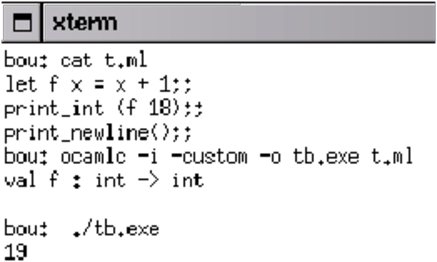
\includegraphics {img/session_with_bytecode_compiler}}
	\caption{\label{fig:session_with_bytecode_compiler}Пример работы с байт--код
компилятором}
\end{figure}

\subsection{Нативный компилятор}

Принцип действия компилятора машинного кода такой же что и байт--код
компилятора, с разницей в сгенерированных файлах. Большинство опций компиляции
те же что проведены в таблицах
\ref{tbl:principal_options_of_the_bytecode_compiler} и
\ref{tbl:other_options_for_the_bytecode_compiler}. Однако, в таблице
\ref{tbl:other_options_for_the_bytecode_compiler} необходимо удалить опции
связанные \ref{tbl:options_specific_to_the_native_compiler}. Уровни
предупреждений остаются теми же.

\begin{table}
	\begin{tabular}{|l|l|}
	\hline
	\texttt{-compact} & оптимизация размера кода \\
	\hline
	\texttt{-S} & сохранить код на ассемблере в файле \\
	\hline
	\texttt{-inline} \it{уровень} & установить {\it уровень} \enq{агрессивности}
разложения функций \\
	\hline
	\end{tabular}
	\caption{\label{tbl:options_specific_to_the_native_compiler}Специальные
опции для нативного компилятора}
\end{table}

Встраивание является улучшенным методом макроподстановки на стадии
препроцессирования. Оно заменяет вызов функции, подставляя тело функции, в
случае когда аргументы определены. Таким образом несколько вызовов функции
соответствуют новым копиям ее тела. Разложением мы избавляемся от затрат,
возникающих при инициализации вызова и возврата функции. Однако, расплатой за
это будет увеличение размера кода. Основные уровни разложения функции следующие:

\begin{itemize}
	\item $0$: разложение разрешено, в случае если оно не увеличивает размер
кода
	\item $1$: значение по умолчанию, при этом допускается небольшое увеличение
кода
	\item $n > 1$: увеличивает терпимость к увеличению кода 
\end{itemize}

\subsection{Интерактивный интерпретатор}

У интерактивного интерпретатора всего две опции:

\begin{itemize}
	\item \texttt{-I} {\it каталог}: добавить каталог в начало списка каталогов,
где находятся
скомпилированные файлы или исходники.
	\item \texttt{-unsafe}: не проверять выход индекса за пределы для векторов и
строк
\end{itemize}

Интерактивный интерпретатор распознает несколько директив, позволяющих
интерактивно изменить его функционирование. Все эти директивы описаны в таблице
\ref{tbl:toplevel_loop_directives}, они начинается с символа \texttt{`\#'} и
заканчиваются привычным \texttt{`;;'}.

\begin{table}
	\begin{tabular}{|l|l|}
	\hline
	\texttt{\#quit ;;} & выйти из интерпретатора \\
	\hline
	\texttt{\#directory} {\it каталог} \texttt{;;} & добавить каталог в список
путей \\
	\hline
	\texttt{\#cd каталог} \texttt{;;} & сменить текущий каталог \\
	\hline
	\texttt{\#load} {\it объектный\_файл} \texttt{;;} & загрузить файл .cmo \\
	\hline
	\texttt{\#use} {\it исходный\_файл} \texttt{;;} & скомпилировать и загрузить
исходных файл \\
	\hline
	\texttt{\#print\_depth} {\it глубина} \texttt{;;} & изменить глубину вывода
на экран \\
	\hline
	\texttt{\#print\_length} {\it ширина} \texttt{;;} & аналогично для ширины \\
	\hline
	\texttt{\#install\_printer} {\it функция} \texttt{;;} & указать функцию
вывода на экран \\
	\hline
	\texttt{\#remove\_printer} {\it функция} \texttt{;;} & переключится на
стандартный вывод на экран \\
	\hline
	\texttt{\#trace} {\it функция} \texttt{;;} & трассировка аргументов функции
\\
	\hline
	\texttt{\#untrace} {\it функция} \texttt{;;} & отменить трассировку \\
	\hline
	\texttt{\#untrace\_all ;;} & отменить все трассировки \\
	\hline
	\end{tabular}
	\caption{\label{tbl:toplevel_loop_directives}Директивы интерпретатора}
\end{table}

Директивы, относящиеся к каталогам, подчиняются правилам используемой
операционной системы.

Директивы загрузки имеют отличное от других директив функционирование. Директива
\texttt{\#use} считывает указанный файл, как если бы он был введён интерактивно.
Директива \texttt{\#load} загружает файл с расширением \texttt{.cmo}. В этом
последнем случае, глобальные декларации этого файла недоступны напрямую. Для
этого необходимо использовать синтаксис с точкой. Если в файле
\texttt{exemple.m} содержится глобальное объявление \texttt{f}, то после
загрузки байт--код ( \texttt{\#load "example.cmo";;}), значение \texttt{f}
доступно как \texttt{Example.f}. Обратите внимание, что первая буква файла ---
заглавная. Этот синтаксис происходит из модульной системы Objective CAML (см.
главу \ref{??}). Директивы настройки глубины и ширины вывода на экран позволяют
контролировать формат выводимых значений, что удобно, когда мы имеем дело с
большими данными.

Директивы трассировки аргументов и результата функции особенно полезны при
отладке программ. Этот вариант использования интерактивного интерпретатора
рассматривается более подробно в главе об анализе программ (\ref{??}).

На рисунке \ref{fig:session_with_the_toplevel_loop} изображён сеанс работы в
интерпретаторе.

\begin{figure}[h]
	\center{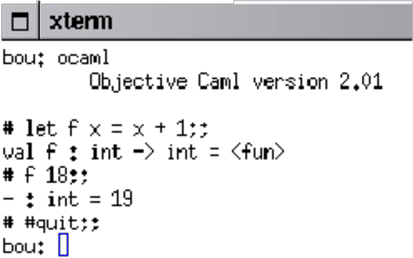
\includegraphics {img/session_with_the_toplevel_loop}}
	\caption{\label{fig:session_with_the_toplevel_loop}Сеанс работы в
интерпретаторе}
\end{figure}

\subsection{Создание интерпретатора}

При помощи команды \texttt{ocamlmktop} мы можем создать новый цикл
интерпретатора, в который загружены определённые библиотеки или модули. Кроме
того, что мы избавляемся от \texttt{\#load} в начале сеанса работы, это так же
необходимо для подключения библиотек на \texttt{C}.

Опции этой команды являются частью опций байт--код компилятора (ocamlc):

$$
-cclib имя\_библиотеки, -ccopt опции, -custom, -I каталог -o имя\_файла
$$

В главе о графическом интерфейсе (4 стр. ??) используется эта команда для
создания цикла содержащего библиотеку Graphics следующим способом:

$$
ocamlmktop -custom -o mytoplevel graphics.cma -cclib \ -I/usr/X11/lib -cclib
-lX11
$$

Эта команда создаёт исполняемый файл \texttt{mytoplevel}, содержащий байт--код
библиотеки \texttt{graphics.cma}. Этот файл является автономным
(-\texttt{custom}, смотрите следующий раздел) и он связан с библиотекой
\texttt{X11 (libX11.a)}, которая располагается в каталоге \texttt{/usr/X11/lib}.